\documentclass[12pt, a4paper]{book}

\usepackage[T1]{fontenc}
\usepackage[utf8]{inputenc}
\usepackage[charter, cal=cmcal]{mathdesign}
\usepackage[scaled=0.92]{helvet}
\usepackage{geometry}
\geometry{a4paper, top=30mm, bottom=30mm, inner=32mm, outer=25mm, marginparwidth=18mm}

\usepackage{amsmath, amsthm}
\usepackage[version=4]{mhchem}
\usepackage{graphicx}
\usepackage{xcolor}
\usepackage{tikz}
\usetikzlibrary{arrows.meta, shapes.geometric, positioning, calc, backgrounds}
\usepackage{pgfplots}
\pgfplotsset{compat=1.18}
\usepackage{tcolorbox}
\tcbuselibrary{skins, breakable, theorems}
\usepackage{titlesec}
\usepackage{fancyhdr}
\usepackage{enumitem}
\usepackage{booktabs}
\usepackage{array}
\usepackage{parskip}
\usepackage{siunitx}
\usepackage[colorlinks=true, linkcolor=BrickRed,
            urlcolor=NavyBlue, citecolor=ForestGreen]{hyperref}

% ── Colours (Journey 2 — charcoal / royal blue) ────────────────────────────────
\definecolor{JourneyColor}{HTML}{0F172A}
\definecolor{ModuleColor}{HTML}{2563EB}
\definecolor{PuzzleColor}{HTML}{D97706}
\definecolor{DiscoveryColor}{HTML}{3B82F6}
\definecolor{WarningColor}{HTML}{991B1B}
\definecolor{ProblemColor}{HTML}{6B21A8}
\definecolor{ReflectColor}{HTML}{0D9488}
\definecolor{HistoryColor}{HTML}{78350F}

% ── Boxes ─────────────────────────────────────────────────────────────────────
\newtcolorbox{puzzlebox}[1][]{enhanced,breakable,
  colback=PuzzleColor!6,colframe=PuzzleColor,fonttitle=\bfseries\sffamily,
  title={The Puzzle},attach boxed title to top left={yshift=-2mm,xshift=6mm},
  boxed title style={colback=PuzzleColor},borderline west={3pt}{0pt}{PuzzleColor},#1}

\newtcolorbox{discoverybox}[1][]{enhanced,breakable,
  colback=DiscoveryColor!8,colframe=DiscoveryColor,fonttitle=\bfseries\sffamily,
  title={Discovery},attach boxed title to top left={yshift=-2mm,xshift=6mm},
  boxed title style={colback=DiscoveryColor},borderline west={3pt}{0pt}{DiscoveryColor},#1}

\newtcolorbox{problembox}[1][]{enhanced,breakable,
  colback=ProblemColor!5,colframe=ProblemColor,fonttitle=\bfseries\sffamily,
  title={Problems},attach boxed title to top left={yshift=-2mm,xshift=6mm},
  boxed title style={colback=ProblemColor},borderline west={3pt}{0pt}{ProblemColor},#1}

\newtcolorbox{deepbox}[1][]{enhanced,breakable,
  colback=JourneyColor!5,colframe=JourneyColor,fonttitle=\bfseries\sffamily,
  title={Deep Problems},attach boxed title to top left={yshift=-2mm,xshift=6mm},
  boxed title style={colback=JourneyColor},borderline west={4pt}{0pt}{JourneyColor},#1}

\newtcolorbox{historybox}[1][]{enhanced,breakable,
  colback=HistoryColor!7,colframe=HistoryColor!60,fonttitle=\bfseries\sffamily\small,
  title={Historical Note},attach boxed title to top left={yshift=-2mm,xshift=6mm},
  boxed title style={colback=HistoryColor!80},#1}

\newtcolorbox{reflectionbox}[1][]{enhanced,breakable,
  colback=ReflectColor!6,colframe=ReflectColor,fonttitle=\bfseries\sffamily,
  title={Reflection},attach boxed title to top left={yshift=-2mm,xshift=6mm},
  boxed title style={colback=ReflectColor},borderline west={3pt}{0pt}{ReflectColor},#1}

\newtcolorbox{namedconcept}[2][]{enhanced,
  colback=ModuleColor!6,colframe=ModuleColor,fonttitle=\bfseries\sffamily\large,
  title={#2},attach boxed title to top left={yshift=-2mm,xshift=6mm},
  boxed title style={colback=ModuleColor},#1}

% ── Section formatting ────────────────────────────────────────────────────────
\titleformat{\chapter}[display]
  {\normalfont\sffamily\huge\bfseries\color{JourneyColor}}
  {\textcolor{JourneyColor!60}{\chaptertitlename\ \thechapter}}{10pt}{\Huge}
  [\vspace{2pt}\textcolor{JourneyColor}{\titlerule[1.5pt]}]
\titleformat{\section}
  {\normalfont\sffamily\Large\bfseries\color{ModuleColor}}
  {\thesection}{1em}{}[\textcolor{ModuleColor!40}{\titlerule[0.6pt]}]
\titleformat{\subsection}
  {\normalfont\sffamily\large\bfseries\color{JourneyColor!80}}{\thesubsection}{1em}{}
\titleformat{\subsubsection}
  {\normalfont\sffamily\normalsize\bfseries}{\thesubsubsection}{1em}{}

\pagestyle{fancy}
\fancyhf{}
\fancyhead[LE]{\small\sffamily\textcolor{JourneyColor}{\leftmark}}
\fancyhead[RO]{\small\sffamily\textcolor{ModuleColor}{\rightmark}}
\fancyfoot[C]{\small\thepage}
\renewcommand{\headrulewidth}{0.4pt}

\newcommand{\newterm}[1]{\textit{\textcolor{DiscoveryColor}{#1}}}
\newcommand{\important}[1]{\textcolor{ModuleColor}{\textbf{#1}}}

\begin{document}

\setcounter{chapter}{1}
\chapter[Journey 2 --- Physical Computation (Silicon to Gate)]
        {Journey Two\\[8pt]
         \textcolor{ModuleColor}{\large Physical Computation (Silicon to Gate)}}
\setcounter{section}{2}

\section{Module 2.3 --- Combinational and Sequential Logic}
\label{sec:mod2.3}

\subsection*{Motivation}

We explored in Module 2.2 how to compile nMOS and pMOS switches into logical CMOS gates, optimizing their delays and power dissipation.
But all the circuits we have designed so far are **combinational**: their output at any instant is determined solely by their current inputs. If we turn off the inputs, the output vanishes.
A computer cannot operate on transient values. It must possess memory: the ability to store a physical state.

This module explores the boundary between static calculations and dynamic state.
We will study combinational blocks like multiplexers and binary adders.
Then, we will introduce **feedback loops**—routing the output of a gate back to its input.
We will discover how cross-coupled gates lock charge in place to form latches, flip-flops, and static RAM cells, providing the physical architecture of computer memory.

\subsection{The Memory Loop}

We investigate how routing output back to input creates a bi-stable system.

\begin{puzzlebox}
\textbf{The Feedback Loop.}

Suppose we connect the output of a logical NOT gate back to its input.
\begin{enumerate}[label=(\alph*), leftmargin=*]
  \item If the propagation delay of the NOT gate is $\tau_d$, explain why the output oscillates continuously between 0 and 1 with a period of $T = 2\tau_d$. (Why is this system unable to store a stable state?)
  \item Now, suppose we connect **two** NOT gates in a closed loop, where the output of the second NOT gate is connected to the input of the first:
  \begin{center}
  \begin{tikzpicture}[scale=1.2]
    \node[draw, shape=triangle, minimum size=0.8cm, rotate=-30] (N1) at (0,0.5) {};
    \fill (-0.4, 0.4) circle (0.05); % inversion bubble
    \node[draw, shape=triangle, minimum size=0.8cm, rotate=150] (N2) at (2,0.5) {};
    \fill (2.4, 0.6) circle (0.05); % inversion bubble
    
    % Connections
    \draw[thick] (0.35,0.5) -- (1.5,0.5);
    \draw[thick] (1.8,0.5) -- (2.3,0.5);
    \draw[thick] (2.3,0.5) -- (2.3, 1.2) -- (-0.3, 1.2) -- (-0.3, 0.5) -- (0.0,0.5);
  \end{tikzpicture}
  \end{center}
        Show that this system has exactly two stable states:
        * State A: Output 1 = 1, Output 2 = 0.
        * State B: Output 1 = 0, Output 2 = 1.
        Why does this cross-coupled inverter loop act as a stable **bi-stable** memory cell, storing a single bit of data?
  \item If the loop is locked in State A, how do we physically force the loop to change to State B? (What addition must we make to the circuit to write new data?)
\end{enumerate}
\end{puzzlebox}

\subsection{Combinational Blocks and Binary Adders}

We construct the processing blocks of the Arithmetic Logic Unit (ALU).

\begin{explobox}
Before storing data, we must process it. We define two primary combinational blocks:
* **Multiplexer (MUX):** Selects one of several input signals based on a select control.
* **Full-Adder:** Computes the arithmetic sum of three binary bits ($A$, $B$, and a carry-in $C_{in}$).
\begin{enumerate}[label=(\alph*), leftmargin=*]
  \item The Boolean equations for a 1-bit Full-Adder sum ($S$) and carry-out ($C_{out}$) are:
  \[
    S \;=\; A \oplus B \oplus C_{in}, \qquad C_{out} \;=\; (A \cdot B) + (C_{in} \cdot (A \oplus B)).
  \]
  Draw the logic gate schematic of the Full-Adder.
  \item Construct a 4-to-1 Multiplexer using basic AND, OR, and NOT gates. The selector lines are $S_1$ and $S_0$.
\end{enumerate}
\end{explobox}

\subsection{Sequential Logic: Latches and Flip-Flops}

We transition from level-sensitive latches to edge-triggered registers.

\begin{explobox}
To write data to our bi-stable loop, we replace the NOT gates with 2-input NOR gates, constructing an **SR Latch** (Set-Reset):
\begin{center}
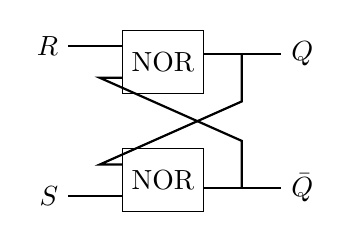
\begin{tikzpicture}[scale=1.0]
  % NOR 1
  \node[draw, minimum size=0.8cm] (NOR1) at (0,1.5) {NOR};
  % NOR 2
  \node[draw, minimum size=0.8cm] (NOR2) at (0,0) {NOR};
  
  \draw[thick] (-1.2, 1.7) -- ($(NOR1.west)+(0,0.2)$) node[left, pos=0] {$R$};
  \draw[thick] (-1.2, -0.2) -- ($(NOR2.west)+(0,-0.2)$) node[left, pos=0] {$S$};
  
  % Outputs
  \draw[thick] ($(NOR1.east)+(0,0.1)$) -- (1.5, 1.6) node[right] {$Q$};
  \draw[thick] ($(NOR2.east)+(0,-0.1)$) -- (1.5, -0.1) node[right] {$\bar{Q}$};
  
  % Cross coupling
  \draw[thick] (1.0, 1.6) -- (1.0, 1.0) -- (-0.8, 0.2) -- ($(NOR2.west)+(0,0.2)$);
  \draw[thick] (1.0, -0.1) -- (1.0, 0.5) -- (-0.8, 1.3) -- ($(NOR1.west)+(0,-0.2)$);
\end{tikzpicture}
\end{center}
\begin{enumerate}[label=(\alph*), leftmargin=*]
  \item Derive the state table for the SR Latch. Show that when $S=0, R=0$, the latch holds its previous state ($Q_{next} = Q$). Show why the input $S=1, R=1$ is invalid (leads to an unstable state when inputs are removed).
  \item **The D Latch:** Combines the SR Latch with steering gates so that the output $Q$ follows the data input $D$ only when the clock $CLK$ is high. Why is a D latch called **level-sensitive**?
  \item **The D Flip-Flop:** Combines two D Latches in a **Master-Slave** configuration, where the master latch is active when $CLK=0$ and the slave when $CLK=1$.
        Explain why this configuration makes the D Flip-Flop **edge-triggered**, capturing the value of $D$ only on the rising edge of the clock. Why is edge-triggering crucial for synchronizing operations in a processor?
\end{enumerate}
\end{explobox}

\newpage

% ─── Section: Discovery ──────────────────────────────────────────────────────
\section{Part 3 --- Discovery}

\begin{discoverybox}
\textbf{What have we built?}

\textbf{First.} Combinational circuits process transient signals, whereas sequential circuits utilize feedback loops to lock charge and store binary states.

\textbf{Second.} The 1-bit Full-Adder calculates Sum and Carry-out, forming the basic arithmetic building block of the CPU.

\textbf{Third.} The SR Latch is a bi-stable loop that can be Set ($Q=1$) or Reset ($Q=0$), but has an invalid state when both control inputs are active.

\textbf{Fourth.} A D Flip-Flop uses a Master-Slave latch pair to achieve edge-triggering, capturing data only on the clock transition edge. This isolates input noise and synchronizes logic across the clock cycles of a processor.
\end{discoverybox}

\newpage

% ─── Section: Naming Concepts ────────────────────────────────────────────────
\section{Part 4 --- What This Is Called}

\begin{namedconcept}{Logical sequential parameters}
* **Combinational Logic:** Logic circuits whose outputs depend solely on the current inputs.
* **Sequential Logic:** Logic circuits containing memory elements, whose outputs depend on both current inputs and the history of past states.
* **SR Latch:** Set-Reset Latch. A basic asynchronous bi-stable circuit.
* **D Flip-Flop:** Data Flip-Flop. An edge-triggered storage element that captures the input state on a clock edge.
* **Metastability:** An unstable equilibrium state in a bi-stable circuit, where it fails to settle to a stable 0 or 1 within the required time.
\end{namedconcept}

\newpage

% ─── Section: Solved Exercises ───────────────────────────────────────────────
\section{Part 5 --- Solved Exercises}

\begin{problembox}
\begin{enumerate}[label=\textbf{E\arabic*.}]
  \item \textbf{Transition Table of the D Flip-Flop.}
  
        Write down the state transition table of a positive-edge-triggered D Flip-Flop.
        Show how the next state $Q_{n+1}$ depends on the inputs $D$, the clock $CLK$, and the current state $Q_n$.
        
        \textbf{Solution:}
        A positive-edge-triggered D Flip-Flop captures the logic level of the $D$ input only on the rising edge of the clock (transition from 0 to 1, denoted by $\uparrow$).
        At all other times (when $CLK = 0$, $CLK = 1$, or during a falling edge $\downarrow$), the flip-flop ignores the input $D$ and holds its current state $Q_n$.
        
        Let us write the complete state transition table:
        
        \begin{center}
        \begin{tabular}{cccc}
          \toprule
          \textbf{Clock ($CLK$)} & \textbf{Data ($D$)} & \textbf{Current State ($Q_n$)} & \textbf{Next State ($Q_{n+1}$)} \\
          \midrule
          0 & $X$ & 0 & 0 (Hold) \\
          0 & $X$ & 1 & 1 (Hold) \\
          1 & $X$ & 0 & 0 (Hold) \\
          1 & $X$ & 1 & 1 (Hold) \\
          $\downarrow$ & $X$ & 0 & 0 (Hold) \\
          $\downarrow$ & $X$ & 1 & 1 (Hold) \\
          $\uparrow$ & 0 & $X$ & 0 (Reset) \\
          $\uparrow$ & 1 & $X$ & 1 (Set) \\
          \bottomrule
        \end{tabular}
        \end{center}
        Here, $X$ represents a "don't care" state (the value has no effect on the outcome).
        This table demonstrates that the next state $Q_{n+1}$ is completely decoupled from the current state $Q_n$ on a rising clock edge, acting as a clean memory register.
        
  \item \textbf{Implementing XOR Logic with a Multiplexer.}
  
        Show how a 4-to-1 Multiplexer (which selects one of four inputs $I_0, I_1, I_2, I_3$ using select lines $S_1, S_0$) can be configured to execute a 2-input XOR gate ($Y = A \oplus B$).
        
        \textbf{Solution:}
        A 4-to-1 Multiplexer has the output relation:
        \[
          Y \;=\; \overline{S_1}\overline{S_0} I_0 + \overline{S_1} S_0 I_1 + S_1 \overline{S_0} I_2 + S_1 S_0 I_3.
        \]
        The truth table for a 2-input XOR gate ($Y = A \oplus B$) is:
        \begin{center}
        \begin{tabular}{ccc}
          \toprule
          \textbf{$A$} & \textbf{$B$} & \textbf{Output ($Y$)} \\
          \midrule
          0 & 0 & 0 \\
          0 & 1 & 1 \\
          1 & 0 & 1 \\
          1 & 1 & 0 \\
          \bottomrule
        \end{tabular}
        \end{center}
        Let us connect the select lines of the multiplexer to the inputs:
        \[
          S_1 \;=\; A, \qquad S_0 \;=\; B.
        \]
        Substitute these into the multiplexer equation:
        \[
          Y \;=\; \overline{A}\overline{B} I_0 + \overline{A} B I_1 + A \overline{B} I_2 + A B I_3.
        \]
        To match the XOR truth table, we set the inputs to constant voltages representing 0 or 1:
        * For $A=0, B=0$, we want $Y=0 \implies I_0 = 0$ (GND).
        * For $A=0, B=1$, we want $Y=1 \implies I_1 = 1$ ($V_{DD}$).
        * For $A=1, B=0$, we want $Y=1 \implies I_2 = 1$ ($V_{DD}$).
        * For $A=1, B=1$, we want $Y=0 \implies I_3 = 0$ (GND).
        
        Thus, by connecting the inputs as:
        \[
          I_0 \;=\; 0, \qquad I_1 \;=\; 1, \qquad I_2 \;=\; 1, \qquad I_3 \;=\; 0,
        \]
        the 4-to-1 Multiplexer behaves exactly as an XOR gate.
\end{enumerate}
\end{problembox}

\newpage

% ─── Section: Problems ───────────────────────────────────────────────────────
\section{Part 6 --- Problems}

\begin{problembox}
\begin{enumerate}[label=\textbf{P\arabic*.}]
  \item \textbf{The JK Flip-Flop.}
  
        The JK Flip-Flop improves upon the SR latch by eliminating the invalid state. When both inputs are high ($J=1, K=1$), the flip-flop toggles its output state ($Q_{n+1} = \bar{Q}_n$).
        The state transition equation for a JK Flip-Flop is:
        \[
          Q_{n+1} \;=\; J \bar{Q}_n + \bar{K} Q_n.
        \]
        \begin{enumerate}[label=(\alph*)]
          \item Construct the state transition table for the JK Flip-Flop showing the next state $Q_{n+1}$ for all combinations of $J, K$, and $Q_n$.
          \item Show how to construct a positive-edge-triggered D Flip-Flop using a JK Flip-Flop and a single NOT inverter.
        \end{enumerate}

  \item \textbf{Ripple-Carry Adder Delay.}
  
        An $N$-bit binary adder can be constructed by cascading $N$ 1-bit Full-Adders in series, where the carry-out ($C_{out}$) of stage $i$ is connected directly to the carry-in ($C_{in}$) of stage $i+1$. This is a **Ripple-Carry Adder**.
        Let the delay of a 1-bit Full-Adder to compute the carry-out from $C_{in}$ be $\tau_c$, and to compute the sum $S$ from $C_{in}$ be $\tau_s$.
        \begin{enumerate}[label=(\alph*)]
          \item Explain why the addition of two $N$-bit numbers cannot be completed in parallel.
          \item Prove that the worst-case propagation delay for an $N$-bit Ripple-Carry Adder is:
                \[
                  \tau_{\text{delay}} \;=\; (N-1) \tau_c + \tau_s.
                \]
          \item If $\tau_c = \SI{40}{ps}$ and $\tau_s = \SI{60}{ps}$, calculate the delay of a 64-bit Ripple-Carry Adder.
                Why does this carry propagation delay limit the clock speed of an ALU?
        \end{enumerate}
\end{enumerate}
\end{problembox}

\newpage

% ─── Section: Deep Problems ──────────────────────────────────────────────────
\section{Part 7 --- Deep Problems}

\begin{deepbox}
\begin{enumerate}[label=\textbf{D\arabic*.}]
  \item \textbf{Setup and Hold Times and Metastability.}
  
        For an edge-triggered D Flip-Flop to capture data reliably, the data input $D$ must be stable before and after the active clock edge.
        * **Setup Time ($t_{su}$):** The minimum time $D$ must be stable *before* the clock edge.
        * **Hold Time ($t_h$):** The minimum time $D$ must be stable *after* the clock edge.
        If these times are violated, the internal feedback loop of the flip-flop can be left in an unstable intermediate state (both inverters at $V_{DD}/2$), a state called **metastability**.
        
        \begin{enumerate}[label=(\alph*)]
          \item Let the Master-Slave D Flip-Flop consist of a Master D-latch (transmission gate delay $t_{tg}$, inverter loop delay $t_{inv}$) and a Slave D-latch.
                Explain the physical origin of the setup time $t_{su}$. (Why must the data arrive early enough to propagate through the Master latch's loop before the clock switches the input transmission gate OFF?)
          \item Derive an expression for $t_{su}$ in terms of the internal gate delays $t_{tg}$ and $t_{inv}$.
          \item Once a flip-flop enters a metastable state, the voltage difference $\Delta V(t)$ between the cross-coupled nodes grows exponentially due to positive feedback:
                \[
                  \Delta V(t) \;=\; \Delta V_0 \cdot e^{\frac{t}{\tau_s}},
                \]
                where $\tau_s$ is the time constant of the inverter loop.
                If the logic threshold is $V_{DD}/2 \pm V_{\text{noise}}$, calculate the time $T_{\text{settle}}$ required for the flip-flop to settle to a valid logic level as a function of the initial noise offset $\Delta V_0$.
                Why does a smaller initial offset (coming from a worse setup-time violation) make the settling time exponentially longer?
        \end{enumerate}

  \item \textbf{SRAM Cell Stability and the Butterfly Curve.}
  
        A Static Random-Access Memory (SRAM) cell stores a single bit using a 6-transistor (6T) cell, consisting of a cross-coupled CMOS inverter loop and two access transistors connected to Bit Lines.
        During a **read** operation, the access transistors turn ON, which can pull up the voltage of the node storing "0" slightly.
        If this voltage rises above the threshold of the opposite inverter, the cell will flip its state, erasing the data!
        
        \begin{enumerate}[label=(\alph*)]
          \item The stability of the SRAM cell is analyzed by plotting the **Voltage Transfer Characteristics (VTC)** of the two cross-coupled inverters.
                Inverter 1: $V_2 = f(V_1)$.
                Inverter 2: $V_1 = f(V_2)$.
                Overlay these two curves on a single plot ($V_2$ vs $V_1$), creating the **Butterfly Curve**.
          \item The **Static Noise Margin (SNM)** is defined as the maximum noise voltage that can be introduced at the inverter inputs without flipping the state.
                Explain how the SNM is represented geometrically on the Butterfly Curve as the side length of the largest square that can be nested inside the "eyes" of the butterfly.
          \item During a read, the access transistor act as a voltage divider with the pull-down nMOS of the inverter.
                Explain why making the pull-down nMOS transistor wider (decreasing its resistance) compared to the access transistor increases the SNM, making the cell more stable.
        \end{enumerate}
\end{enumerate}
\end{deepbox}

\newpage

% ─── Section: Reflection ─────────────────────────────────────────────────────
\section{Part 8 --- Reflection}

\begin{reflectionbox}
\textbf{Conceptual Reflection}

Consider the following questions:
\begin{enumerate}
  \item **On the Nature of Memory:** A logic gate has no memory because its outputs are determined purely by current inputs. Memory only emerges when we route the output back into the input (feedback). Is memory, therefore, not a property of material substances, but a property of circular geometry?
  \item **On Synchronous Order:** A processor uses a global clock to synchronize billions of flip-flops. Without this clock, differences in path delays would cause signals to arrive at different times, leading to logical chaos. Why does computation require this periodic, artificial time structure to maintain order?
  \item **On Metastability as Indecision:** A metastable flip-flop is the physical equivalent of "Buridan's Ass"—a hungry donkey placed exactly halfway between two identical bales of hay, unable to choose and starving to death. How does positive feedback resolve this physical indecision, and why does it always require a non-zero time to do so?
\end{enumerate}
\end{reflectionbox}

\medskip
\noindent\textbf{Looking ahead.}
Module~2.4 introduces **Processor Architecture and Memory Hierarchies**. Having built adders to process data and flip-flops to store state, we will connect them to construct a complete processor: registers, instruction decoding, cache hierarchies, and main memory.

\vspace{1.4cm}
\begin{center}
{\color{JourneyColor}\rule{0.5\linewidth}{0.8pt}}\\[6pt]
{\small\color{JourneyColor}\textit{End of Journey 2, Module 2.3 --- Combinational and Sequential Logic}}\\[4pt]
{\small\color{JourneyColor}Continue to: \textbf{Module 2.4 --- Processor Architecture and Memory Hierarchies}}\\[6pt]
{\color{JourneyColor}\rule{0.5\linewidth}{0.8pt}}
\end{center}

\end{document}
